\section{Motivation \& Grundlagen}

\begin{frame}
    \frametitle{Motivation}

    \begin{itemize}
        \item bisher: strukturierte Daten in Form von Zahlenwerten in Tabellen oder Datensätzen
        \item aber: 80\% aller Geschäftsdaten liegen als unstrukturierte oder semi-strukturierte Daten ohne bzw. ohne festes Schema vor
    \end{itemize}   

    \vspace*{1cm}
    {\small
    \begin{notebox}
    Text mining, text data mining (TDM) or text analytics is the process of deriving high-quality information from text. It involves "the discovery by computer of new, previously unknown information, by automatically extracting information from different written resources."\\
    \xspace [Source: Wikipedia]
    \end{notebox}
    }

\end{frame}

%----------------------------------------------------

\begin{frame}[c]
    \frametitle{Motivation: Anwendungsgebiete}

    \begin{center}
    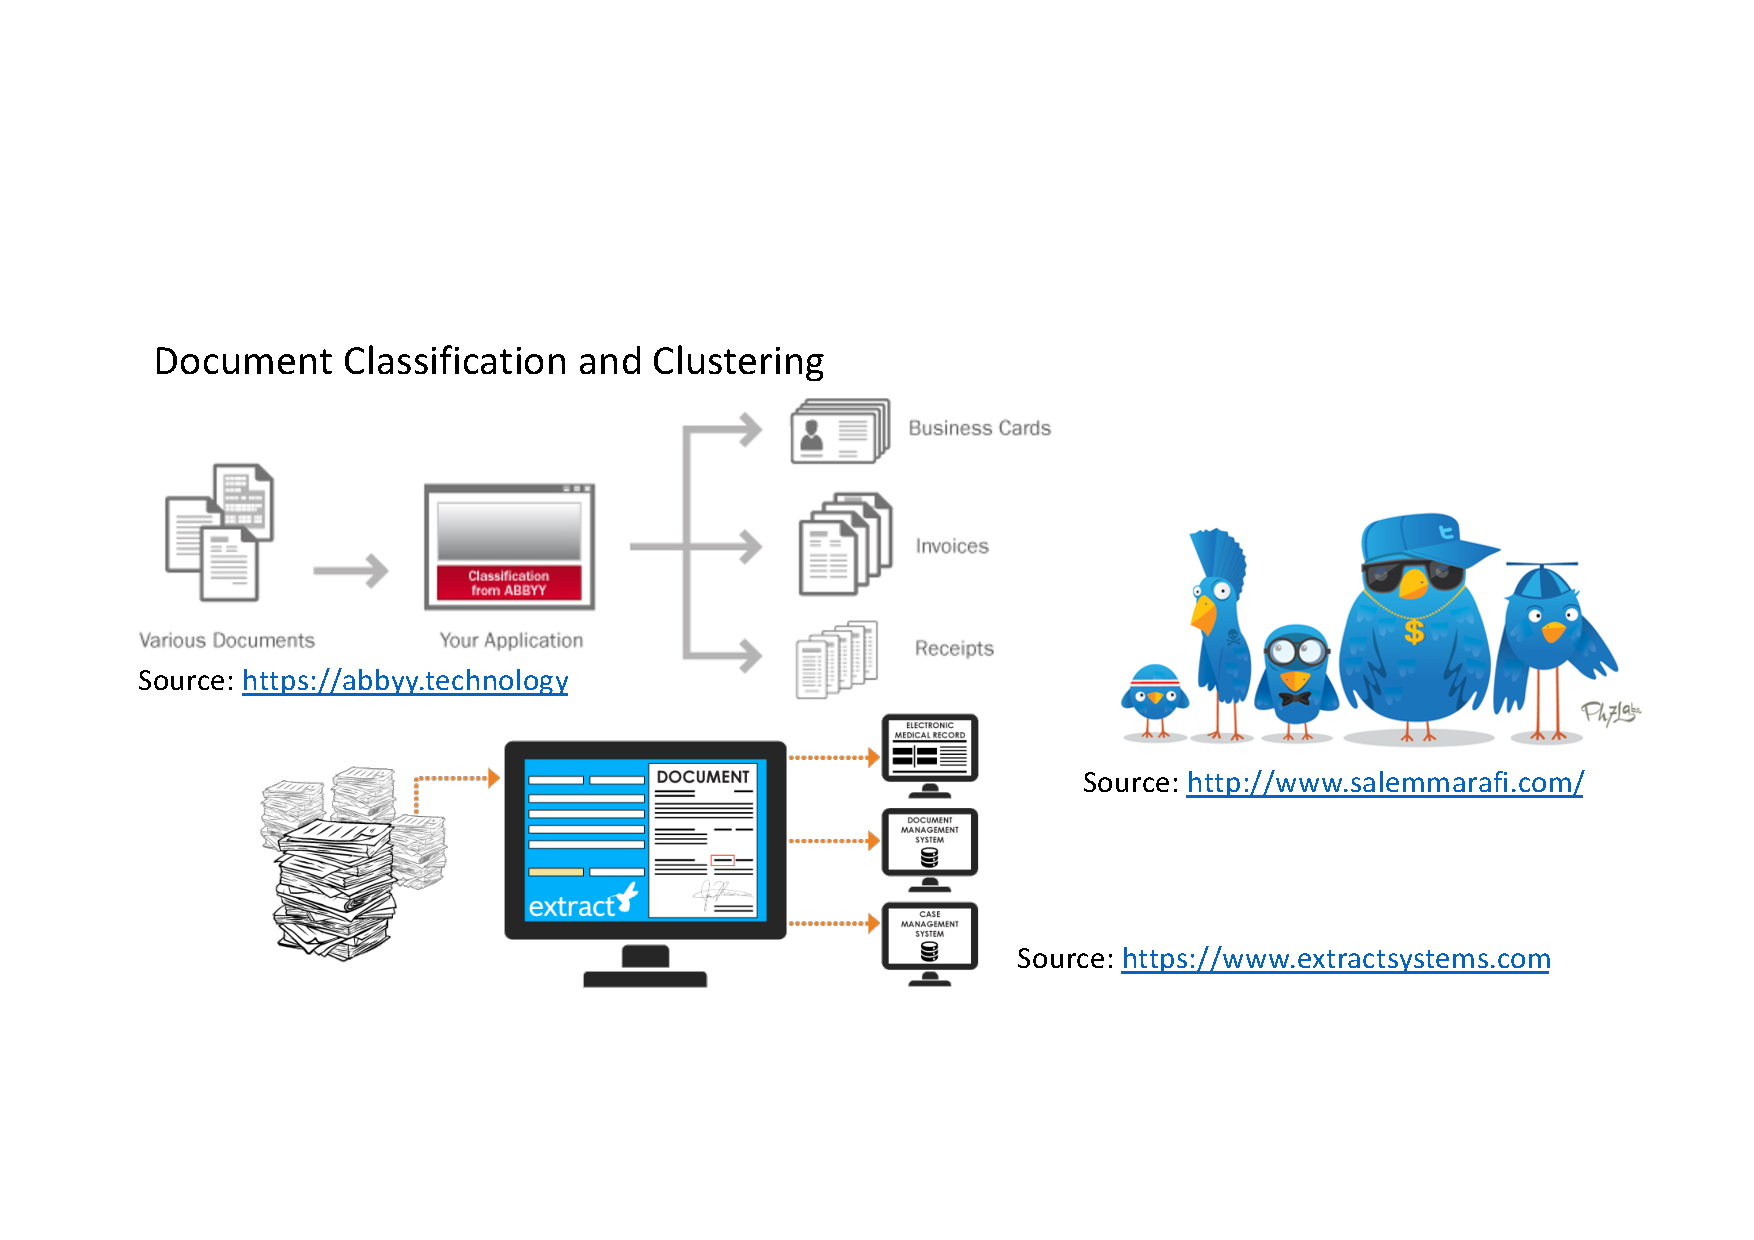
\includegraphics[width=\textwidth]{fig8/motivation-1.pdf}
    \end{center}

\small{Thanks to Michael Gertz: Text Analytics WS 2020/21, Uni Heidelberg}
\end{frame}

%----------------------------------------------------

\begin{frame}[c]
    \frametitle{Motivation: Anwendungsgebiete /2}

    \centering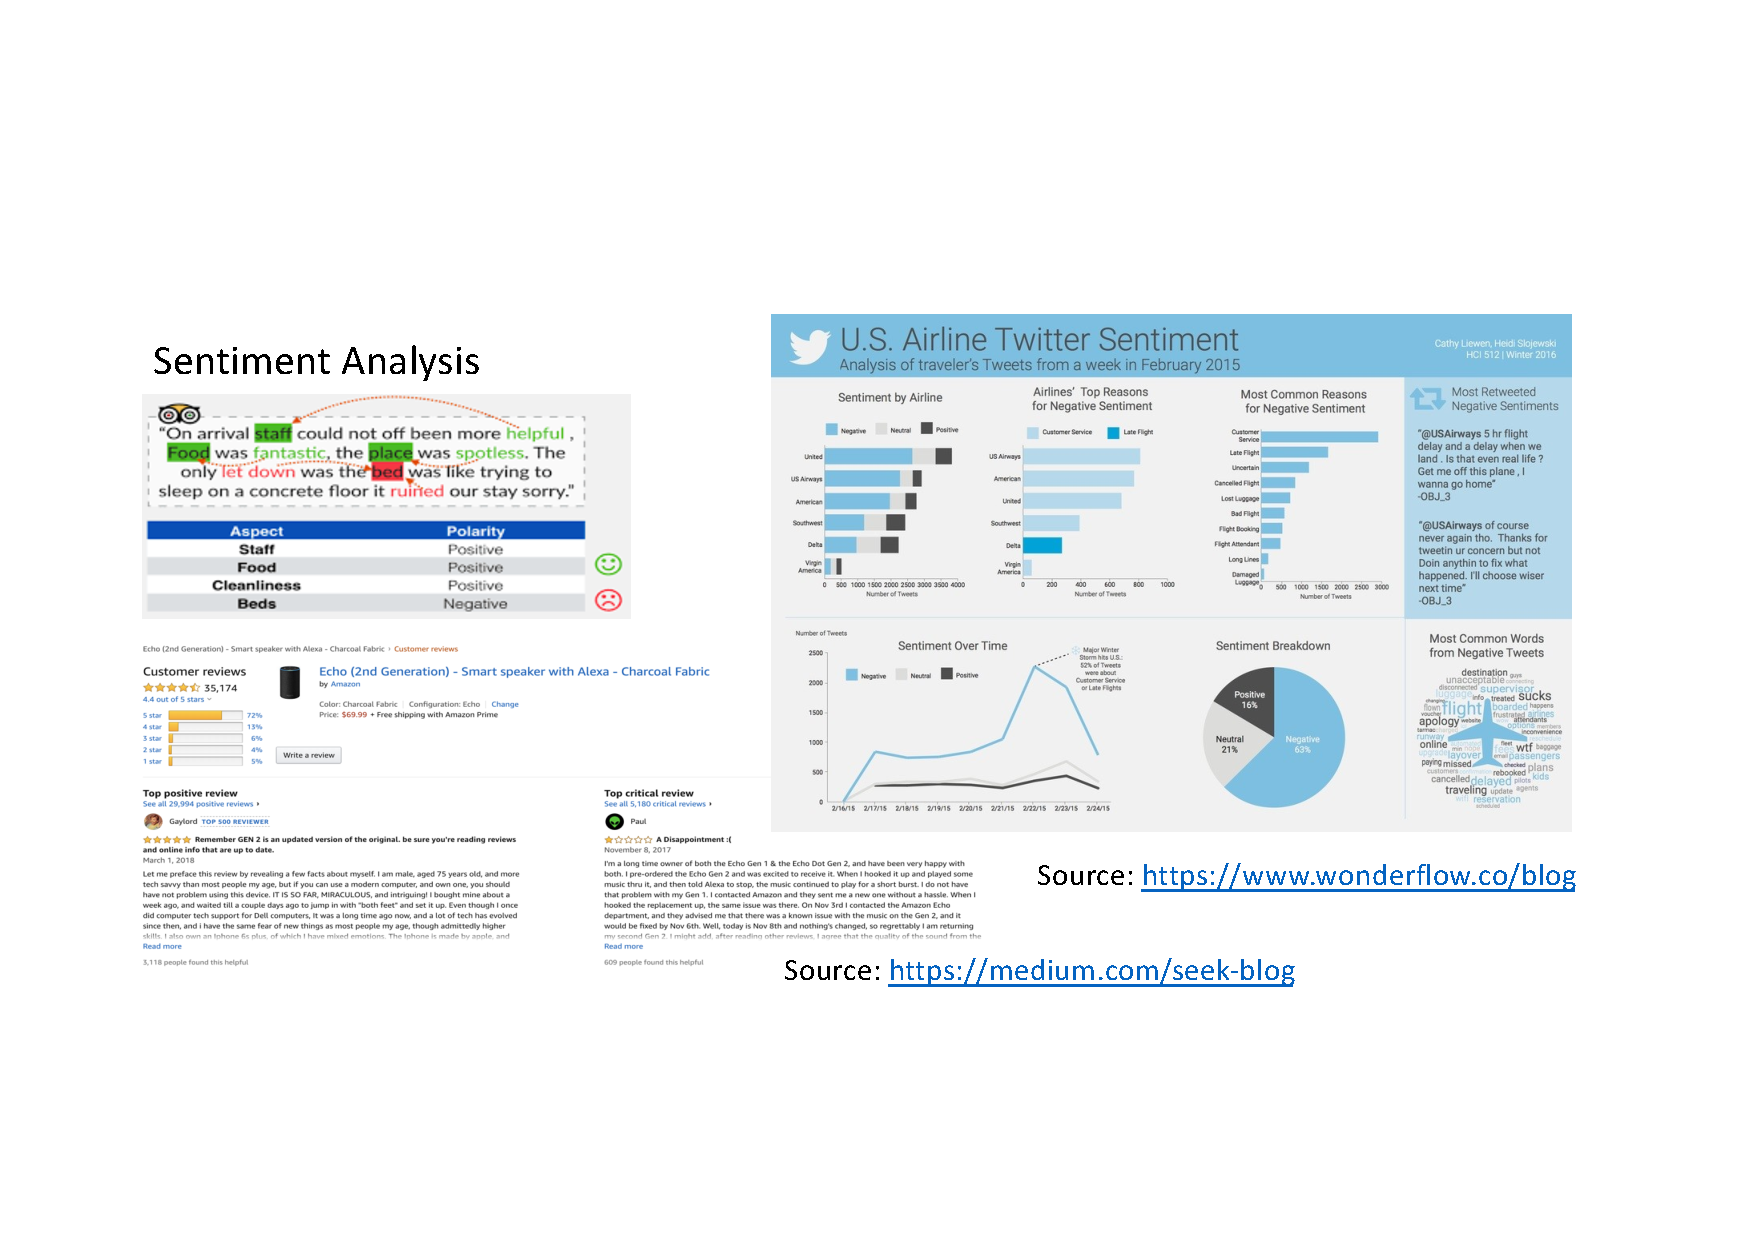
\includegraphics[width=\textwidth]{fig8/motivation-2.pdf}
\end{frame}

%----------------------------------------------------

\begin{frame}[c]
    \frametitle{Motivation: Anwendungsgebiete /3}

    \centering\includegraphics[width=\textwidth]{fig8/motivation-3.pdf}
\end{frame}

%----------------------------------------------------

\begin{frame}[c]
    \frametitle{Motivation: Anwendungsgebiete /4}

    \centering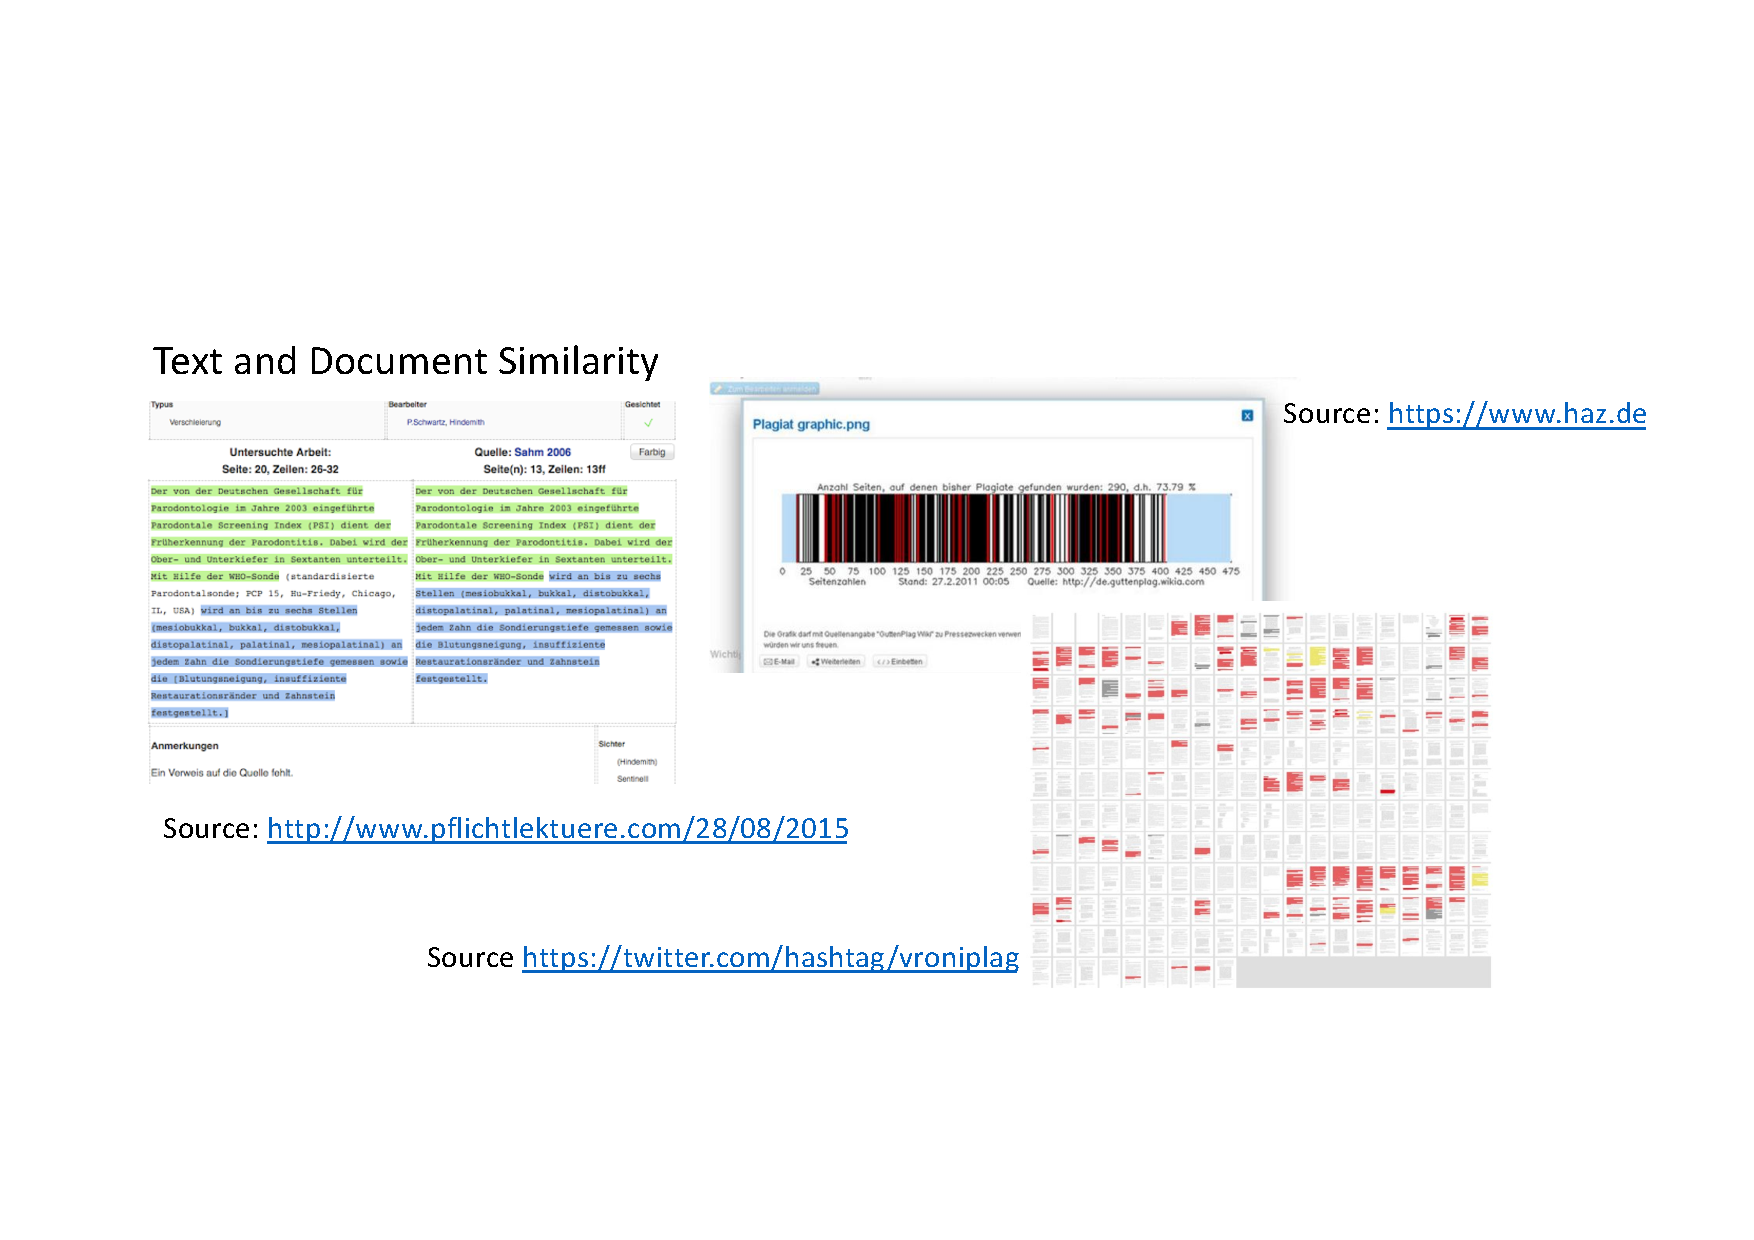
\includegraphics[width=\textwidth]{fig8/motivation-4.pdf}
\end{frame}

%----------------------------------------------------

\begin{frame}[c]
    \frametitle{Motivation: Anwendungsgebiete -- NLP}

    \centering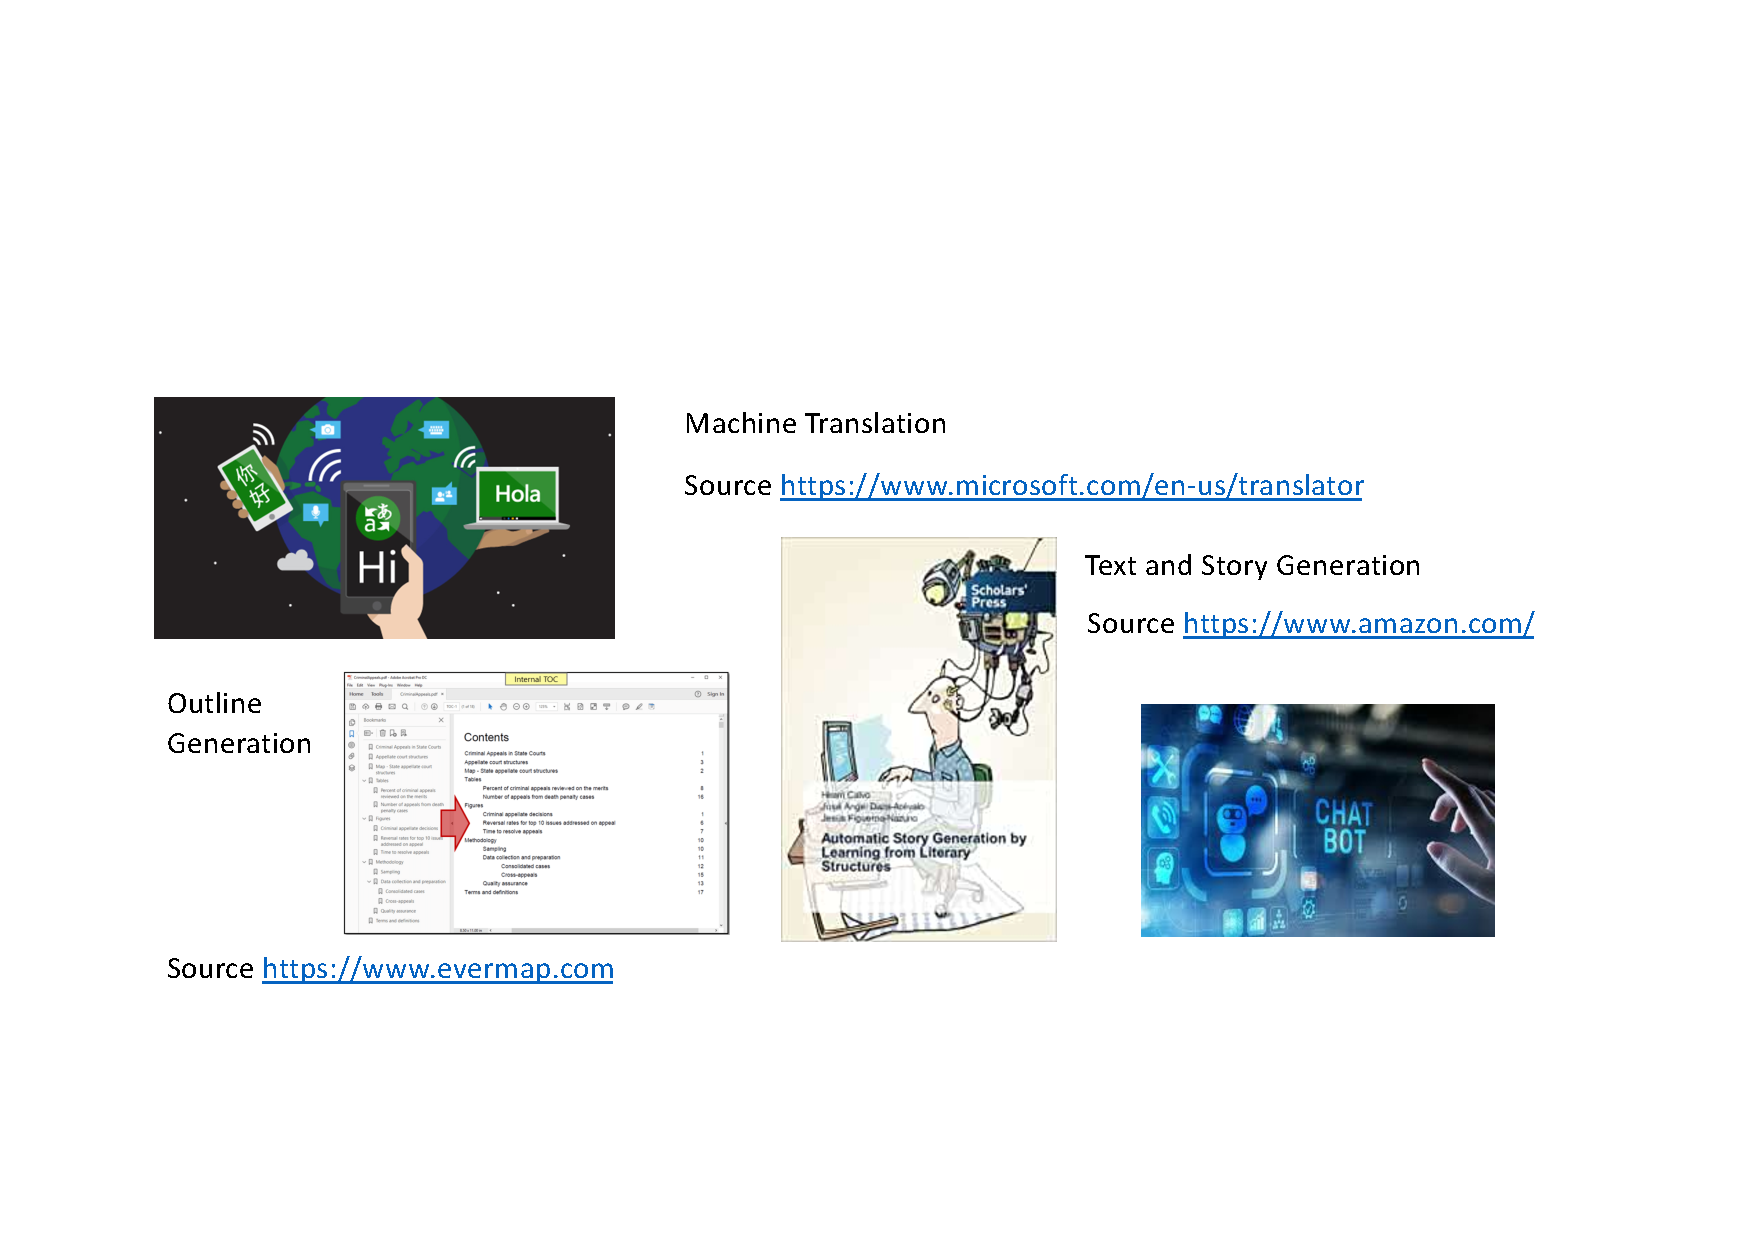
\includegraphics[width=\textwidth]{fig8/motivation-5.pdf}
\end{frame}

%----------------------------------------------------

\begin{frame}
    \frametitle{Textanalyse: Grundlagen}

    für die meisten der genannten Anwendungsfälle sind geeignete Textanalyse-Pipelines und -Komponenten essentiell:

    \begin{itemize}
    \item Textvorverarbeitung (Tokenisierung, Normalisierung, \dots)
    \item Textrepräsentation (Vektorraum-Modell, Worteinbettung, \dots)
    \item Textähnlichkeitsmetriken
    \item skalierbare Architekturen für effiziente Verarbeitung großer Datenmengen
    \end{itemize}

    gilt auch für Suchmaschinen, Chatbots, Sprachmodelle, \dots
    %1-24
\end{frame}

%----------------------------------------------------

\begin{frame}
    \frametitle{Textanalyse: Herausforderungen}

    \begin{itemize}
        \item natürliche Sprache ist \hl{symbolbasiert} und \hl{diskret}, mit Grundelementen (Zeichen), aus denen Wörter gebildet werden, die Objekte, Konzepte, Aktionen, Ereignisse etc. bezeichnen
        \item Wörter sind \hl{eindeutige} Symbole, d.h. es besteht keine inhärente Beziehung zwischen den Wörtern
        \item Sprache ist \hl{kompositional}: Buchstaben bilden Wörter, Wörter bilden Phrasen und Sätze
        $\leadsto$ Bedeutung einer Phrase ist mehr als die Bedeutung einzelner Wörter
    \end{itemize}
   

\end{frame}
%----------------------------------------------------
\begin{frame}
    \frametitle{Textanalyse: Herausforderungen /2}

    \begin{columns}[c]
        \begin{column}{4cm}
    
\includegraphics[width=4cm]{fig8/ntv.png}
        \end{column}
        \begin{column}{4cm}
    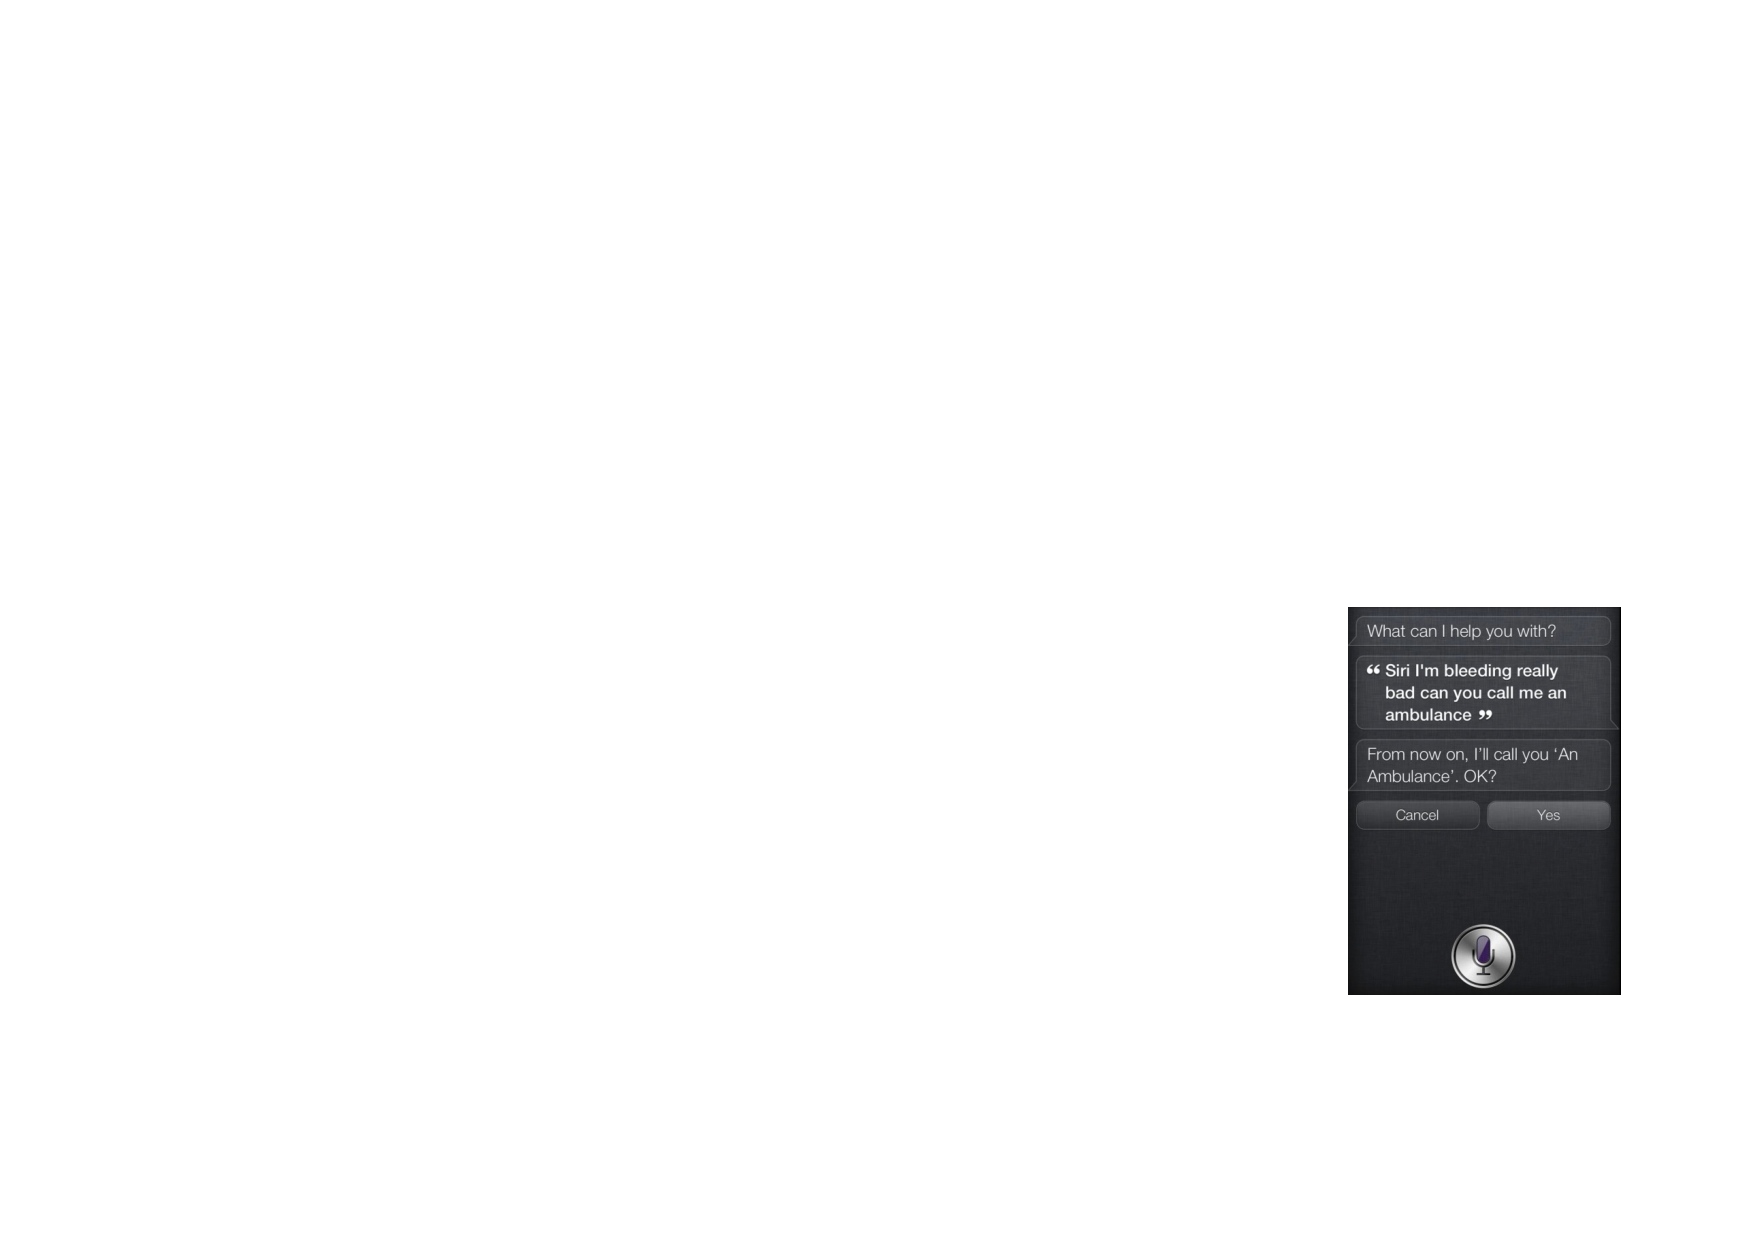
\includegraphics[width=3.5cm]{fig8/siri.pdf}
        \end{column}
    \end{columns}

\end{frame}
%----------------------------------------------------

\section{Vorverarbeitung von Textdokumenten}

%----------------------------------------------------

\begin{frame}[c]
    \frametitle{Textvorverarbeitung: Überblick}

\centering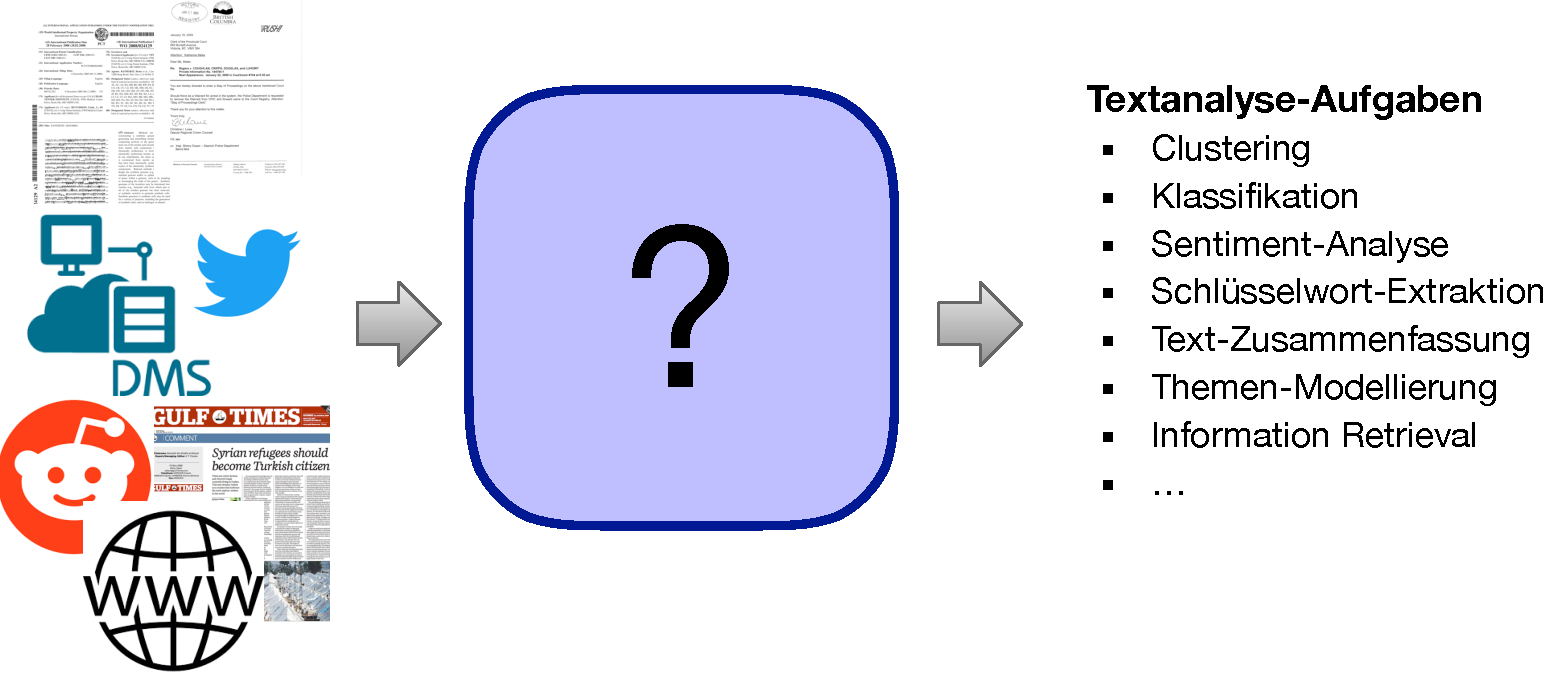
\includegraphics[width=\textwidth]{fig8/text-overview.pdf}

\end{frame}

%----------------------------------------------------

\begin{frame}[shrink=10]
    \frametitle{Textdaten}

    \hl{Aufgabe:} Konvertierung von Rohtext in Zeichenfolge
    $\leadsto$ einfach, wenn Dokumente bereits in reinen Textformaten vorliegen

    \textbf{Binärformate:}
    \begin{itemize}
    \item Portable Document Format (PDF)
    \item Microsoft Office format (.doc[x], .ppt[x], .xls[x])
    \item diverse Werkzeuge und Bibliotheken für Konvertierung, z.B. pdf2text, docx (Python), \dots 
    \end{itemize}
    \textbf{Web and Semi-strukturierte Daten:}
    \begin{itemize}
    \item HTML, XML, JSON
    \item umfasst Metadaten zu Stil und Struktur (Entfernen oder Aufbewahren?)
     \end{itemize}
    \textbf{Zeichensatzkodierung:} Unicode, UTF-8, UTF-16, ASMO 708, GBK, \dots
    
\end{frame}


%----------------------------------------------------

\begin{frame}
    \frametitle{Textvorverarbeitung: Schritte}

    \centering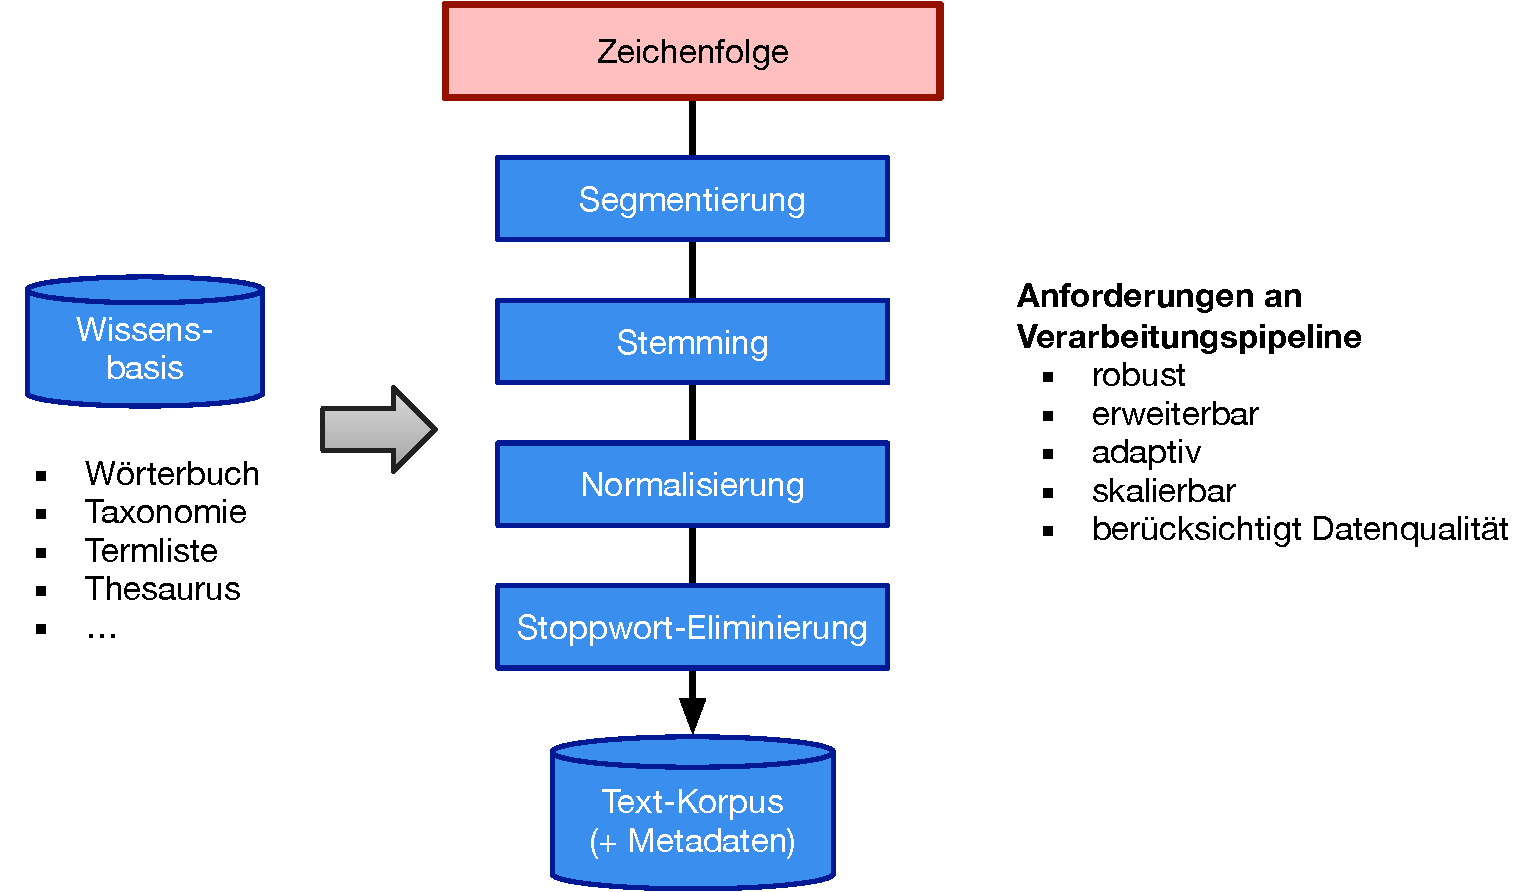
\includegraphics[width=\textwidth]{fig8/text-preprocessing.pdf}

% Abbildung ähnlich 2-24
\end{frame}

%----------------------------------------------------

\begin{frame}
    \frametitle{Tokenisierung / Segmentierung}
    
    \hl{Ziel}: Zerlegung von Sätzen und Wörtern in Elemente (Segmente)

    Unterscheidung nach Granularität und Typ:
    \begin{itemize}
    \item Word Tokenizer
    \begin{itemize}
        \item TreebankWordTokenizer -- unter Verwendung von regulären Ausdrücken, orientiert sich an der Penn Treebank
        \item WordPunctTokenizer -- Trennung eines Textes in alphabetische und nicht-alphabetische Zeichen, ebenfalls unter Verwendung eines regulären Ausdrucks
        \item WhitespaceTokenizer -- Trennung eines Textes am Leerzeichen
    \end{itemize}
    \item Sentence Detection -- (intelligente) Satzerkennung (Stichwort: Interpunktion)
    \end{itemize}
\end{frame}
    
%---------------------------------------------------------------------
    
\begin{frame}[fragile]
    \frametitle{Segmentierung: Treebank Word Tokenizer}
    
    \begin{minted}{python}
    import nltk
    # nur beim ersten Verwenden von nltk -
    # laden der trainierten classifier und dictionaries: 
    # nltk.download('all') 
    from nltk.tokenize import word_tokenize
    text="I can't put my hat back on."
    print(word_tokenize(text))
    \end{minted}

    \texttt{$[$'I', 'ca', "n't", 'put', 'my', 'hat', 'back', 'on', '.'$]$}
\end{frame}
    
%---------------------------------------------------------------------
    
\begin{frame}[fragile]
    \frametitle{Segmentierung: Word Punct Tokenizer}
    
    \begin{minted}{python}
    from nltk.tokenize import WordPunctTokenizer 
    s = 'I can't put my hat back on.' 
    WordPunctTokenizer().tokenize(s)
    \end{minted}

    \texttt{$[$'I', 'can', \dq ' \dq, 't', 'put', 'my', 'hat', 'back', 'on', '.'$]$}
\end{frame}
    
 %---------------------------------------------------------------------
    
\begin{frame}[fragile]
    \frametitle{Segmentierung: Whitespace Tokenizer}
   
   \begin{minted}{python}
    from nltk.tokenize import WhitespaceTokenizer
    s = 'I can't put my hat back on.'
    WhitespaceTokenizer().tokenize(s)
    \end{minted}

    \texttt{$[$'I', "can't", 'put', 'my', 'hat', 'back', 'on.'$]$}
\end{frame}
 
%---------------------------------------------------------------------
    
\begin{frame}[fragile]
    \frametitle{Segmentierung: Sentence Detection}
    
    \begin{minted}{python}
    from nltk.tokenize import sent_tokenize
    text = 'I can't put  my hat back on. Mr. X told me so.'
    print(sent_tokenize(text))
    \end{minted}

    \texttt{$[$'I can't put  my hat back on.', 'Mr. X told me so.'$]$}
\end{frame}
    
%----------------------------------------------------

\begin{frame}
    \frametitle{Stemming / Lemmatisierung}
    \hl{Ziel:} unterschiedlich flektierte Wortformen sollen als gleiches Wort (Lexem) erkannt werden
    
    \textbf{Lemmatisierung}
    \begin{itemize}
    \item Ziel: Ermittle das Lemma (Grundform, Zitierform)
    \item Vollformenlexikon
    \item linguistische Analyse der morphologischen Wortuntereinheiten + Lookup 
    \end{itemize}
    Beispiel: 
    fliegt, flog, geflogen etc. $\rightarrow$ fliegen
\end{frame}
    
%---------------------------------------------------------------------
    
\begin{frame}[fragile]
    \frametitle{Lemmatisierung}


    \begin{minted}{python}
    from nltk.stem import WordNetLemmatizer 
    lemmatizer = WordNetLemmatizer()
    print(lemmatizer.lemmatize("corpora"))
    print(lemmatizer.lemmatize("better", pos ='a'))
    \end{minted}

    Deutsch:
    \begin{minted}{python}
    from HanTa import HanoverTagger as ht
    hannover = ht.HanoverTagger('morphmodel_ger.pgz')
    print(hannover.analyze('geflogen'))
    \end{minted}
\end{frame}
    
%---------------------------------------------------------------------
    
\begin{frame}
    \frametitle{Stemming / Lemmatisierung}

    \textbf{Stemming}
    \begin{itemize}
    \item Ziel: Zurückführung von Wörtern auf (künstlichen) Wortstamm
    \item regel-basierter/heuristischer Ansatz
    \item simple Transformationsregeln
    \end{itemize}

    Beispiele: \\
    Museen $\rightarrow$ Muse\\
    essen $\rightarrow$ ess
    
\end{frame}
    
%---------------------------------------------------------------------
    
\begin{frame}[fragile]
    \frametitle{Stemming}

    \begin{minted}{python}
    from nltk.stem.snowball import SnowballStemmer
    snowball = SnowballStemmer("english")
    print ('Snowball: ' + snowball.stem('museum'))
    \end{minted}

    Deutsch:
    \begin{minted}{python}
    from nltk.stem.snowball import SnowballStemmer
    snowball = SnowballStemmer("german")
    print ('Snowball: ' + snowball.stem('Museen'))
    \end{minted}
    \end{frame}
    
    %---------------------------------------------------------------------
    
    \begin{frame}
    \frametitle{Weiteres}
    Weitere Normalisierung:

    \begin{itemize}
    \item Groß- und Kleinschreibung
    \item Schreibfehler korrigieren
    \item Stoppwörter entfernen
    \end{itemize}
\end{frame}
     
%----------------------------------------------------
\begin{frame}
    \frametitle{Stoppwort-Eliminierung}

    \hl{Ziel:} Entfernen nicht-relevanter/semantikarmer Wörter

    \centering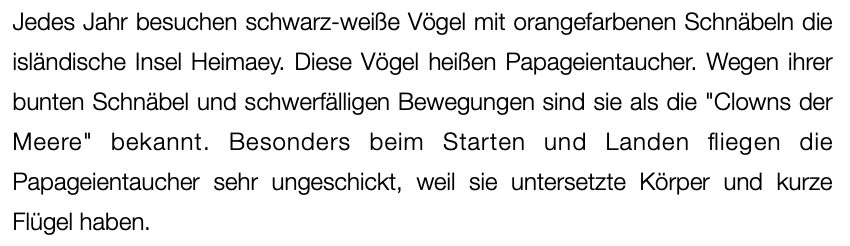
\includegraphics[width=\textwidth]{fig8/stopwords_example1}

\end{frame}
     
%----------------------------------------------------
\begin{frame}
    \frametitle{Stoppwort-Eliminierung}

    \hl{Ziel:} Entfernen nicht-relevanter/semantikarmer Wörter

    \centering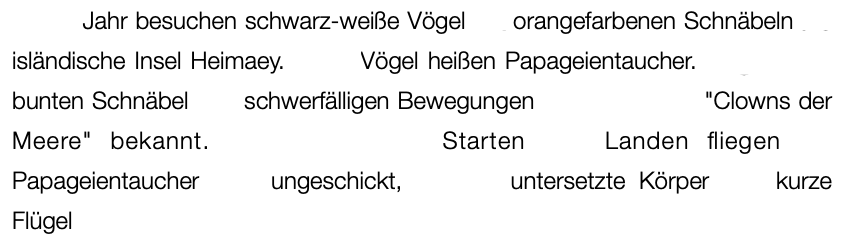
\includegraphics[width=\textwidth]{fig8/stopwords_example2}

\end{frame}
     
%----------------------------------------------------

\begin{frame}[fragile]
    \frametitle{Stoppwort-Eliminierung}

\begin{minted}{python}
    import nltk
    from nltk.corpus import stopwords
    nltk.download('stopwords')
    from nltk.tokenize import word_tokenize
    example = "This is a sample sentence 
        I created to remove stopwords."
    tokens = word_tokenize(example)
    wo_stopwords = [word for word in tokens 
        if not word in stopwords.words()]
    \end{minted}

    \texttt{$[$'This', 'sample', 'sentence', 'I', 'created', 'remove', 'stopwords', '.'$]$}
    
\end{frame}

%----------------------------------------------------

\section{Textrepräsentation}

%----------------------------------------------------
\
\begin{frame}
    \frametitle{Motivation}

    \begin{itemize}
    \item Steigende Anzahl von Dokumenten: im Web, auf dem eigenen Computer, in Content-Management-Systemen von Unternehmen etc.
    \item Fragestellung: Welche Dokumente gehören zusammen/sind ähnlich?
    \item Use Case -- Emails:
    \begin{itemize}
    \item Spam
    \item Arbeit
    \item Privat
    \end{itemize}
    \item Use Case -- Buchrezensionen:
    \begin{itemize}
    \item Gute Bewertung
    \item Schlechte Bewertung
    \end{itemize}
    \end{itemize}
\end{frame}

%----------------------------------------------------

\begin{frame}
    \frametitle{Motivation /2}

\hl{Ziel:} Abbildung von Textelementebn in einen einheitlichen Semantikraum zur Unterstützung effizienter, skalierbarer numerischer Berechnung
als Basis für verschiedene Textanalyseaufgaben

% Bild von Michael
\end{frame}

 %---------------------------------------------------------------------
    
\begin{frame}
    \frametitle{Motivation /3}
    
    \begin{table}[htp]
    \begin{center}
    \begin{tabular}{p{5cm}p{5cm}}
    \tiny{\textbf{tagesschau.de: So kam der Mensch auf die Katze}} & \tiny{\textbf{welt.de: Wie Katzen unsere Sofas eroberten}} \\
    \hline
    \tiny{Forscher haben das Geheimnis der Abstammung der Hauskatzen gelüftet. Für ihre Studie untersuchten die Wissenschaftler die DNA von 230 Tieren aus aller Welt. Darunter waren Tiere aus steinzeitlichen Fundstätten, aber auch Mumien aus dem alten Ägypten und Überreste aus Wikingergräbern. Die Biologen und Archäologen extrahierten die DNA aus Knochen und Zähnen und verglichen die Proben dann mit dem Genmaterial heutiger Hauskatzen. Das verblüffende Ergebnis: "Alle Hauskatzen stammen von einer wilden Rasse ab, die sich Felis silvestris lybica nennt“.} & \tiny{Um die Geschichte der heutigen Stubentiger zu klären, hat ein internationales Forscherteam die sterblichen Überreste von mehr als 200 Katzen analysiert. Diese stammten von archäologischen Funden aus dem Nahen Osten, Ägypten und aus Wikingergräbern. Aus Knochen, Zähnen und Fell extrahierten die Wissenschaftler DNA und verglichen diese mit Genmaterial heutiger Hauskatzen. Dabei stellten sie fest, dass alle domestizierten Katzen von nur einer wilden Art abstammen: der Falbkatze oder Afrikanischen Wildkatze Felis silvestris lybica.}\\
    
    \end{tabular}
    \end{center}
    \end{table}%
\end{frame}
    
%---------------------------------------------------------------------
    
    \begin{frame}
    \frametitle{Motivation /3}
    \begin{center}
    \scriptsize{\textbf{Terme in beiden Texten (abzüglich Stoppwörtern):\\knochen, extrahierten, wikingergräbern, dna, hauskatzen, silvestris, ägypten, zähnen, überreste, felis, genmaterial, lybica, verglichen, wilden, wissenschaftler}}
    \end{center}
    
    \begin{table}[htp]
    \begin{center}
    \begin{tabular}{p{5cm}p{5cm}}
    \multicolumn{2}{c}{\scriptsize{\textbf{Terme in jeweils nur einem der Texte (abzüglich Stoppwörtern):}}}\\
    \scriptsize{stammen, rasse, forscher, 230, studie, alten, ergebnis, fundstätten, gelüftet, proben, untersuchten, steinzeitlichen, geheimnis, archäologen, mumien, tiere, biologen, verblüffende, welt, tieren, abstammung} & \scriptsize{internationales, funden, katzen, abstammen, domestizierten, forscherteam, sterblichen, 200, falbkatze, analysiert, fest, fell, stubentiger, afrikanischen, art, archäologischen, klären, osten, stammten, geschichte, wildkatze} \\
    \end{tabular}
    \end{center}
    \end{table}%
    
\end{frame}
    
%----------------------------------------------------

\begin{frame}[fragile]
    \frametitle{Bag-of-Words-Modell}

    Bag-of-Words = Liste aller Terme, die in einem Text enthalten sind - ungeordnet und ohne weitere Features.

    \begin{minted}{python}
    import nltk
    from nltk.tokenize import sent_tokenize
    from nltk.tokenize import WordPunctTokenizer
    wpt = WordPunctTokenizer()

    from nltk.corpus import stopwords
    nltk.download('stopwords')

    text = "Forscher haben das [...] lybica nennt."
    sentences = sent_tokenize(text)
    \end{minted}
\end{frame}

\begin{frame}[fragile]
    \frametitle{Bag-of-Words-Modell}
     
    \begin{minted}{python}
    words = []
    punctuation = [".",",",":"]
    for sentence in sentences:
        sentence = str.lower(sentence)
        word_list = wpt.tokenize(sentence)
        wo_sw = [word for word in word_list if not word in 
            stopwords.words('german')]
        wo_sw_punct = [word for word in wo_sw if word
            not in punctuation]
        words.extend(wo_sw_punct)          
    words = sorted(list(set(words)))
    \end{minted}
\end{frame}
    
 %---------------------------------------------------------------------
    
\begin{frame}
    \frametitle{Vektorraum-Modell}
    \begin{itemize}
    \item Repräsentation jedes Dokuments als Vektor
    \item jeder Term eines Dokuments stellt eine Dimension dar 
    \item Zum Vergleich mehrerer Dokumente benötigt:
    \begin{itemize}
    \item Basis-Vektor („Vokabular“, „Lexikon“, „Dictionary“) der alle Terme aller Dokumente enthält
    \item jeder Dokumenten-Vektor benutzt als Referenz den Basis-Vektor, im Dokument vorhandene Terme aus dem 
    Vokabular werden im Vektor markiert
    \end{itemize}
    \end{itemize}
\end{frame}
    
%---------------------------------------------------------------------
    
\begin{frame}
    \frametitle{Vektorraum-Modell}
    \begin{itemize}
    \item Dokument 1 enthält 40 verschiedene Terme, Dokument 2 enthält 42 verschiedene Terme
    \item Gemeinsames Vokabular aus beiden Texten enthält 66 Terme -- Basisvektor hat 66 Dimensionen
    \item jeder Dokumentenvektor hat ebenfalls 66 Dimensionen
    \item verschiedene Möglichkeiten Vorkommen eines Terms im Dokument zu markieren:
    \begin{itemize}
    \item binär - 0/1  $\rightarrow$ Term kommt vor oder nicht
    \item Termhäufigkeit  $\rightarrow$ Anzahl des Vorkommens des Terms im Dokument
    \item TF*IDF  $\rightarrow$ gewichtetes Vorkommen
    \end{itemize}
    \end{itemize}
\end{frame}
    
%---------------------------------------------------------------------
    
\begin{frame}
    \frametitle{Vektorraum-Modell}
    \vspace{1.5cm}
    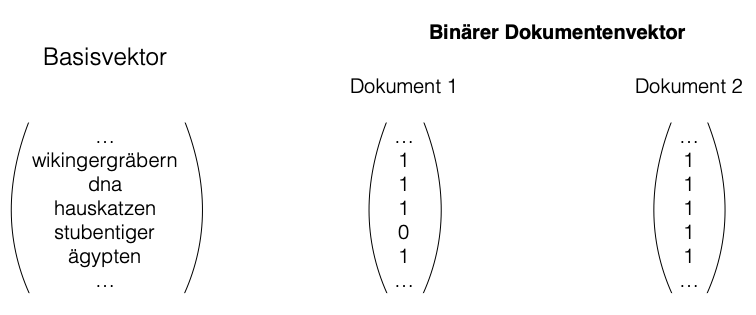
\includegraphics[width=\linewidth]{fig8/binaervektor}
    $\leadsto$ One-Hot-Encoding
\end{frame}
    
%---------------------------------------------------------------------
    
\begin{frame}[fragile]
    \frametitle{Vektorraum-Modell}
    
    \begin{minted}{python}
    from sklearn.feature_extraction.text import CountVectorizer
    vectorizer = CountVectorizer(binary=True)
    vectors = vectorizer.fit_transform([words,words2])
    feature_names = vectorizer.get_feature_names()
    dense = vectors.todense()
    denselist = dense.tolist()
    df = pd.DataFrame(denselist, columns=feature_names)
    \end{minted}
\end{frame}
      
 %---------------------------------------------------------------------
    
\begin{frame}
    \frametitle{Vektorraum-Modell}
    \vspace{1.5cm}
    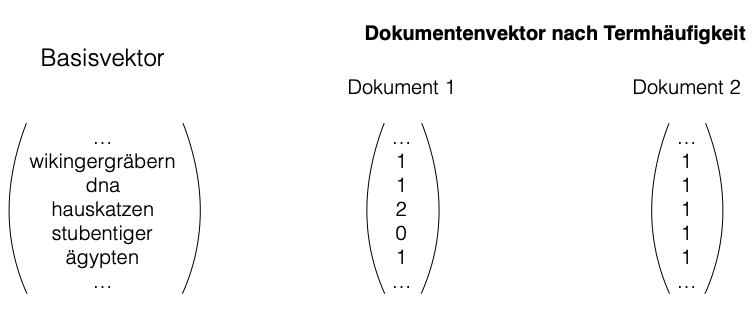
\includegraphics[width=\linewidth]{fig8/tfvektor}
    
\end{frame}


%---------------------------------------------------------------------
    
\begin{frame}
    \frametitle{Vektorraum-Modell}
    \vspace{.5cm}
    
    \begin{table}[htp]
    \begin{center}
    \begin{tabular}{p{3cm}p{7cm}}
    \multicolumn{2}{c}{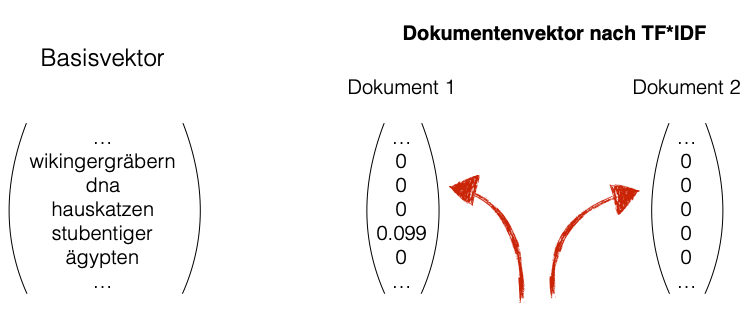
\includegraphics[width=\linewidth]{fig8/tfidfvektor}}\\
     & \tiny{Die Werte sind 0, da der log(1)=0 -> die Terme kommen in allen Dokumenten des Korpus (bestehend aus diesen zwei Dokumenten) vor und sind daher nicht relevant für das einzelne Dokument (siehe Berechnung IDF)}\\
    \end{tabular}
    \end{center}
    \end{table}
    
\end{frame}
    
%---------------------------------------------------------------------
    
\begin{frame}[fragile]
\frametitle{Vektorraum-Modell}
    
    \begin{minted}{python}
    from sklearn.feature_extraction.text import TfidfVectorizer
    vectorizer = TfidfVectorizer()
    vectors = vectorizer.fit_transform([words,words2])
    feature_names = vectorizer.get_feature_names()
    dense = vectors.todense()
    denselist = dense.tolist()
    df = pd.DataFrame(denselist, columns=feature_names)
    \end{minted}
\end{frame}
     
%---------------------------------------------------------------------
    
\begin{frame}
    \frametitle{Vektorraum-Modell: Ähnlichkeitsmaß}
    Vergleich von Dokumenten:
    Welches Dokument ist der Anfrage am ähnlichsten?
    \vspace{0.3cm}
    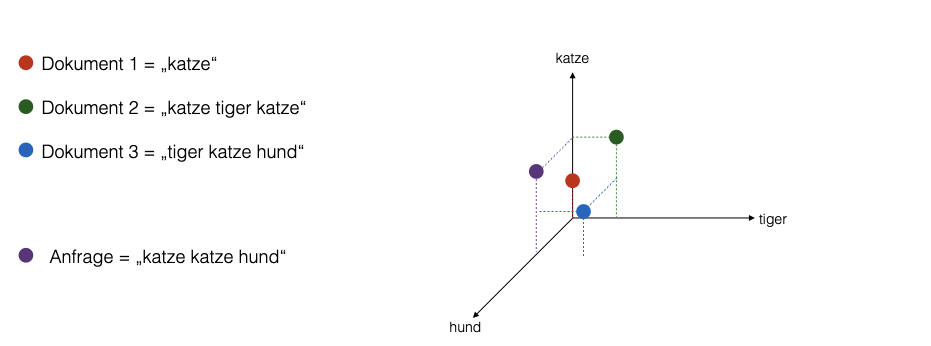
\includegraphics[width=\linewidth]{fig8/vector_space}
    
\end{frame}
    
%---------------------------------------------------------------------
    
\begin{frame}
\frametitle{Vektorraum-Modell: Ähnlichkeitsmaß}
    Vergleich von Dokumenten:
    Welches Dokument ist der Anfrage am ähnlichsten?
    \vspace{0.3cm}
    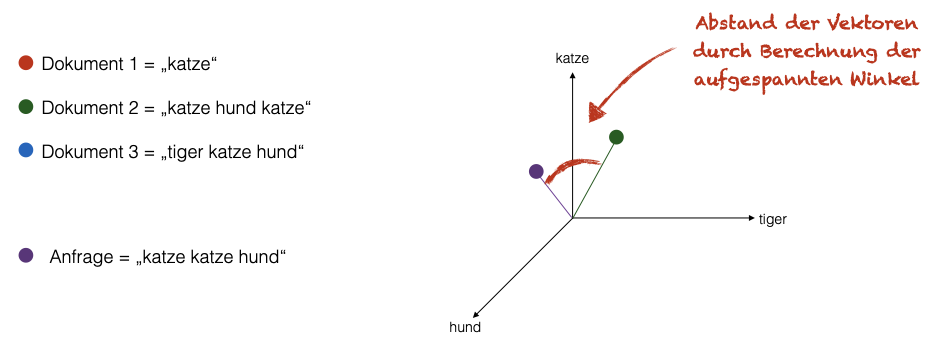
\includegraphics[width=\linewidth]{fig8/vector_space_distance}
    \scriptsize{Abstand der Vektoren ergibt Ähnlichkeitsmaß zwischen verschiedenen Dokumenten\\
    Häufiges Maß: Cosinus-Similarity - durch Berechnung des Kosinus des Winkels wird Normierung des Ähnlichkeitsmaß auf Werte zwischen 0 und 1 erreicht.\\
    Kosinus-Ähnlichkeit = 1 $\rightarrow$ Vektoren liegen übereinander (maximale Ähnlichkeit) \\
    Kosinus-Ähnlichkeit = 0  $\rightarrow$ Vektoren liegen orthogonal zueinander (keine Ähnlichkeit) }
    
\end{frame}
    
%---------------------------------------------------------------------
    
\begin{frame}[fragile]
    \frametitle{Vektorraum-Modell: Ähnlichkeitsmaß}
    Vergleich von Dokumenten: Kosinus-Abstand als Ähnlichkeitsmaß zweier Vektoren.

    \begin{minted}{python}
    from scipy import spatial
    # convert data frame to array to extract separate vectors
    arr = df.to_numpy()
    # compute distance between vectors:
    cos = 1 - spatial.distance.cosine(arr[0],arr[1])
    \end{minted}

    \begin{itemize}
    \item Wenn  Distanz 0 ist $\rightarrow$ Ähnlichkeit am größten 
    \item Daher muss die Distanz von 1 abgezogen werden
    \end{itemize}
\end{frame}
 
%----------------------------------------------------

\section{Klassifikation \& Clustering}


\begin{frame}
    \frametitle{Klassifikation von Texten}

    Genereller Ansatz bei Klassifikation von Textdokumenten:
    \begin{itemize}
    \item Gegeben ist eine Menge von Dokumenten D und eine Menge von definierten Klassen C. Der (Text) Klassifikator ist eine Funktion f:D $\rightarrow$ C
    \item Vorgehensweise (1/2):
    \begin{itemize}
    \item Dokument D wird in Feature-Vektor V umgewandelt mithilfe Funktion v (bspw. mit TF*IDF gewichteten Termen) (\textbf{Feature Space})
    \item Erstellung eines Trainingsdatensatzes mit Dokumentvektoren und zugeordneten Klassen (\textbf{Trainingsdaten})
    \end{itemize}
    \end{itemize}
\end{frame}
    
%---------------------------------------------------------------------

\begin{frame}
    \frametitle{Klassifikation von Texten}

    Genereller Ansatz bei Klassifikation von Textdokumenten:
    \begin{itemize}
    \item Vorgehensweise (2/2):
    \begin{itemize}
    \item Definition der Charakteristiken der Dokumente, die derselben Klasse zugeordnet sind (\textbf{Modell})
    \begin{itemize}
    \item was haben sie gemeinsam?
    \item Wie unterscheiden sie sich von Dokumenten in anderen Klassen?
    \end{itemize}
    \item Modell wird in Klassifikator überführt, der den Feature-Vektor prozessiert:
    \begin{itemize}
    \item v: D $\rightarrow$ V
    \item f : V $\rightarrow$ C
    \end{itemize}
    \item Berechnet wird: f(v(D))
    \end{itemize}
    \end{itemize}
\end{frame}
    
%---------------------------------------------------------------------
    
\begin{frame}
    \frametitle{Klassifikation von Texten}
 
    Für das Training des Klassifikators sind verschiedene Algorithmen möglich:\\
    \begin{itemize}
    \item Nearest Neighbor
    \item Naïve Bayes
    \item Maximum Entropy 
    \item Support Vector Machines
    \item etc.
    \end{itemize}
    
\end{frame}
    
%---------------------------------------------------------------------
    
\begin{frame}[fragile]
    \frametitle{Klassifikation von Texten: Beispiel mit SVM}
    
    \begin{minted}{python}
    from sklearn.datasets import fetch_20newsgroups
    categories = ['comp.graphics', 'sci.med']
    train = fetch_20newsgroups(subset='train',
        categories=categories, shuffle=True, random_state=42)
    from sklearn.feature_extraction.text import CountVectorizer
    count_vect = CountVectorizer()
    X_train_counts = count_vect.fit_transform(train.data)
    tfidft= TfidfTransformer()
    X_train_tfidf = tfidft.fit_transform(X_train_counts)
    \end{minted}
\end{frame}
    
%---------------------------------------------------------------------
    
\begin{frame}[fragile]
    \frametitle{Klassifikation von Texten: Beispiel mit SVM}
    
    \begin{minted}{python}
    from sklearn import svm
    clf = svm.SVC()
    clf.fit(X_train_tfidf, train.target)
    docs_new = ['Covid-19 is a bad disease.', 
        'OpenGL on the GPU is fast']
    X_new_counts = count_vect.transform(docs_new)
    X_new_tfidf = tfidft.transform(X_new_counts)
    predicted = clf.predict(X_new_tfidf)
    
    for doc, category in zip(docs_new, predicted):
        print('\%r => \%s' % (doc, train.target_names[category]))
    \end{minted}
    
    \texttt{'Covid-19 is a bad disease.' => sci.med}\\
    \texttt{'OpenGL on the GPU is fast' => comp.graphics}
    
\end{frame}
    
%---------------------------------------------------------------------

\begin{frame}[fragile]
    \frametitle{Clustering}

    \begin{minted}{python}
    from sklearn.cluster import KMeans
    import numpy as np
    categories = ['sci.space','rec.sport.baseball',
        'comp.graphics','sci.med']
    dataset = fetch_20newsgroups(subset='all', 
        categories=categories, shuffle=True, random_state=42)
    labels = dataset.target
    true_k = np.unique(labels).shape[0]
    vectorizer = TfidfVectorizer(max_df=0.5,
        max_features=10000, min_df=2, stop_words='english', 
        use_idf=True)
    X = vectorizer.fit_transform(dataset.data)
    km = KMeans(n_clusters=true_k, init='k-means++',
        max_iter=100, n_init=1, verbose=False)
    km.fit(X)
    \end{minted}
\end{frame}
    
%---------------------------------------------------------------------
    
 
    
\section{Worteinbettung \& Sprachmodelle}

\section{Anwendungsfälle: Sentimentanalyse, Schlüsselwort-Extraktion, Topic Modeling}